\documentclass[10pt]{article}

\usepackage{graphicx}
\usepackage{amsmath}
\usepackage{amssymb}
%\usepackage{gensymb}
\usepackage{mathtools}
\usepackage{etoolbox}
\usepackage{booktabs}
\usepackage[parfill]{parskip}
\usepackage[numbers]{natbib}
\usepackage{float}
\usepackage{graphicx}
\usepackage{geometry}
\usepackage{multicol}
\usepackage{caption}
\usepackage{url}

\newcommand\mgin{0.5in}
\geometry{
    left=\mgin,
    right=\mgin,
    bottom=\mgin,
    top=\mgin
}

% Set path to import figures from
\graphicspath{{../../img/sparsity/}}

% Place converted graphics in current directory
\usepackage[outdir=./]{epstopdf}

% Define multicolumn figure-like environment
% from http://tex.stackexchange.com/questions/12262/multicol-and-figures
\newenvironment{mcfig}
    {\par\medskip\noindent\minipage{\linewidth}}
    {\endminipage\par\medskip}

% Define error function for math mode
\newcommand{\erf}{\mbox{erf}}
% Sign function
\newcommand{\sign}{\mbox{sign}}
% Natural numbers
\newcommand\N{\mathbb{N}}
% Real numbers
\newcommand\R{\mathbb{R}}
% Complex numbers
\newcommand\C{\mathbb{C}}
% Curly B for basis
\newcommand\BB{\mathcal{B}}
% Curly D for diagonal dominance quantity
\newcommand\DD{\mathcal{D}}
\newcommand\QQ{\mathcal{Q}}
% Curly R for range (not real numbers)
\newcommand\RR{\mathcal{R}}
% Curly N for null space
\newcommand\NN{\mathcal{N}}
% Norm
\newcommand\norm[1]{\left\lVert #1 \right\rVert}
% Uniform Norm
\newcommand\unorm[1]{\left\lVert #1 \right\rVert_\infty}
% Inner Product
\newcommand\ip[1]{\left\langle #1 \right\rangle}
% Absolute value
\newcommand\abs[1]{\left| #1 \right|}
% Complex Conjugate
\newcommand\conj\overline
% Partial derivative
\newcommand\pd[2]{\frac{\partial #1}{\partial #2}}
% Iteration superscript w/ parentheses
\newcommand{\iter}[1]{^{(#1)}}
% Disable paragraph indentation
\setlength{\parindent}{0pt}
% End of proof
\newcommand\qed{\hfill$\blacksquare$\hspace{0.5in}}

% Number this equation
\newcommand\eqnum{\addtocounter{equation}{1}\tag{\theequation}}

% arara: pdflatex
% arara: bibtex
% arara: pdflatex
% arara: pdflatex
\begin{document}

%%fakesection Title
\null

\thispagestyle{empty}
\addtocounter{page}{-1}

\begin{center}
    \begin{sffamily}
    \begin{bfseries}
        \null
        \vfill
        \Huge{Survey of Solution Techniques for Linear Systems from Finite Difference Methods in 2D Numerical Radiative Transfer}

        \vspace{20pt}
        \LARGE{Advanced Numerical Analysis II Final Project} \\
        \vspace{20pt}
    \begin{Large}
        Oliver Evans \\
        Fred Weiss \\
        Christopher Parker \\
        Emmanuel Arkoh \\[1em]

        Dr. Malena Espa\~nol \\
    \vspace{20pt}
    \today
    \end{Large}
    \end{bfseries}
    \end{sffamily}
    \vspace{30pt}

    \null
    \vfill
    \vfill
    \null
\end{center}
\pagebreak


% Increase table cell height (not for header)
\renewcommand{\arraystretch}{1.5}

\begin{multicols}{2}

\section{Introduction}
We use monochromatic radiative transfer in order to model the light field in an aqueous environment populated by vegetation.
The vegetation (kelp) is modeled by a spatial probability distribution, which we assume to be given.
The two quantities we seek to compute are \textit{radiance} and \textit{irradiance}.
Radiance is the intensity of light in at a particular point in a particular direction, while irradiance is the total light intensity at a point in space, integrated over all angles.
The Radiative Transfer Equation is an integro-partial differential equation for radiance, which has been used primarily in stellar astrophysics; it's application to marine biology is fairly recent \citep{mobley_radiative_2001}.

We study various methods for solving the system of linear equations resulting from discretizing the Radiative Transfer Equation.
In particular, we consider direct methods, stationary iterative methods, and nonstationary iterative methods.
Numerical experiments are performed using Python's \texttt{scipy.sparse} \citep{jones_scipy:_2001} package for sparse linear algebra.
\texttt{IPython} \citep{perez_ipython:_2007} was used for interactive numerical experimentation.

Among those implemented, the nonstationary LGMRES \citep{baker_technique_2005} algorithm is the only algorithm determined to be suitable for this application without further work.
We discuss limitations and potential improvements, including preconditioning, alternative discretization, and reformulation of the RTE.

\subsection{Radiative Transfer}
Let $n$ be the number of spatial dimensions for the problem (i.e., 2 or 3).
Let $x \in \RR^n$.
Let $\Omega$ be the unit sphere in $\RR^n$.
Let $\omega \in \Omega$ be a unit vector in $\RR^n$.
Let $L(x,\omega)$ denote \textit{radiance} position $x$ in the direction $\omega$.
Let $I(x)$ denote \textit{irradiance} at position $x$.
Let $P_k(x)$ be the probability density of kelp at position $x$.
Let $a(x)$ and $b(x)$ denote the absorption and scattering coefficients respectively of the medium, which are both functions of $P_k$.
Let $\beta(\Delta\theta)$ denote the normalized \textit{volume scattering function} or \textit{phase function}, which defines the probability of light scattering at an angle $\Delta\theta$ from it's initial direction in a scattering event.

Then, the Monochromatic Time-Independent Radiative Transfer Equation (RTE) is
\begin{equation}
    \tag{RTE}
    \label{eq:rte}
    \begin{aligned}
        \omega \cdot \nabla_x L(x,\omega) &= -(a(x) + b(x)) L(x,\omega) \\
        &\qquad + b \int_\Omega \beta(\omega \cdot \omega') L(x,\omega')\, d\omega'
    \end{aligned}
\end{equation}

Note that in 2 spatial dimensions, this is a 3-dimensional problem ($x,y,\theta$).
Likewise, in 3 spatial dimensions, it is a 5-dimensional problem ($x,y,z,\theta,\phi$).

In this paper, we consider only the 2-dimensional problem, with the hope that sufficiently robust solution techniques for the 2-dimensional problem will be effective in the solution of the 3-dimensional problem, as well.

\subsection{2D Problem}
\label{sec:2d}
We use the downward-pointing coordinate system shown in figure \ref{fig:coords}, measuring $\theta \in [0,2\pi)$ from the positive $x$ axis towards the positive $y$ axis.
Further, we assume that the problem is given on the rescaled spatial domain $[0,1) \times [0,1)$, where $y=0$ is the air-water interface, and $y$ measures depth from the surface.

\begin{figure}[H]
    \centering
    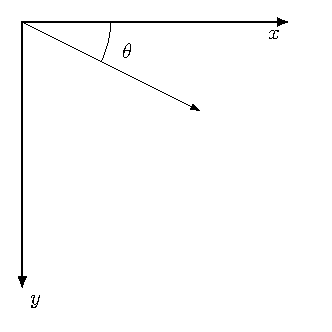
\includegraphics[width=2in]{2d_coords}
    \caption{2D coordinate system}
    \label{fig:coords}
\end{figure}

The 2-dimensional form of \eqref{eq:rte} is given by
\begin{equation}
    \begin{aligned}
        \pd{L}{x} \cos\theta + \pd{L}{y} \sin\theta
        &= -(a+b)L(x,y,\theta) \\
        &+ b\int_0^{2\pi} \beta(\abs{\theta-\theta'})\,d\theta',
    \end{aligned}
    \label{eq:rte2d}
\end{equation}

where $\abs{\theta-\theta'}$ measures the smallest angular difference between $\theta$ and $\theta'$ considering periodicity.

Note that in Cartesian coordinates, there are only spatial, not angular derivatives in the gradient.
In other coordinate systems, this is generally not the case.

\subsection{Boundary Conditions}
We assume that the downwelling light from the surface is known, and is defined to be uniform in space by the Dirichlet boundary condition
\begin{equation}
    L(x,0,\theta) = f(\theta), \quad \mbox{for} \quad \theta \in [0,\pi).
    \label{eq:surf_bc}
\end{equation}

Note that we cannot apply the same idea to upwelling light at the surface, as it cannot be specified from information about the atmospheric light field.
Therefore, we apply the PDE at $y=0$ for $\theta \in [\pi,2\pi)$.

At $y=1$, we assume no upwelling light.
That is,
\begin{equation}
    L(x,0,\theta) = 0, \quad \mbox{for} \quad \theta \in [\pi,2\pi).
    \label{eq:bottom_bc}
\end{equation}

As with the upper $y$-boundary, we apply the PDE for $\theta \in [0,\pi)$ so as not to prohibit downwelling light.

In the horizontal direction, we assume periodic boundary conditions.
Assuming that a single discrete group of plants is being simulated, adjusting the width of the domain effectively modifies the spacing between adjacent groups of plants.

\section{System of Linear Equations}

\subsection{Discretization}
In order to solve \eqref{eq:rte2d} numerically, we discretize the spatial derivatives using 2nd order finite difference approximations, and we discretize the integral according to the Legendre-Gauss quadrature, as described in \citet[Chapter 2]{chandrasekhar_radiative_1960}.
With this in mind, in order to create a spatial-angular grid with $n_x,n_y$, and $n_\theta$ discrete values for $x, y$, and $\theta$ respectively, we use a uniform square spatial discretization with spacing $dx, dy$, and a non-uniform angular discretization according to the roots of the Legendre Polynomial of degree $n_\theta$, denoted $P_{n_\theta}(\theta)$.
In each variable, we discard the uppermost grid point, as indicated by the half-open intervals in the previous sections.

Then, we have the grid
\begin{align}
    x_i &= (i-1)\,dx, &\quad i=1,\ldots,n_x \\
    y_j &= (j-1)\,dy, &\quad j=1,\ldots,n_y \\
    \theta_k \,\, \mbox{s.t.}\,\,
    &P_{n_\theta}(\theta_k/\pi-1) = 0, &\quad k=1,\ldots,n_\theta
\end{align}

In the same notational vein, let \\[-1em]
\begin{align}
    L_{ij}^k &= L(x_i,y_j,\theta_k), \\
    \beta_{kl} &= \beta(\abs{\theta_k-\theta_l}), \\
    a_{ij} &= a(x,y) \\
    b_{ij} &= b(x,y)
\end{align}

where $\abs{\cdot}$ is periodic as in \eqref{eq:rte2d}.

For the spatial interior of the domain, we use the 2nd order central difference formula (CD2) to approximate the derivatives, which is
\begin{equation}
    \tag{CD2}
    f'(x) = \frac{f(x+dx)-f(x-dx)}{2dx} + \mathcal{O}(dx^3).
\end{equation}

When applying the PDE on the upper or lower boundary, we use the forward and backward difference (FD2 and BD2) formulas respectively.
Omitting $\mathcal{O}(dx^3)$, we have
\begin{equation}
    \tag{FD2}
    \label{eq:FD2}
    f'(x) = \frac{-3f(x)+2f(x+dx)-f(x+2dx)}{2dx}
\end{equation}
\begin{equation}
    \tag{BD2}
    \label{eq:BD2}
    f'(x) = \frac{3f(x)-2f(x-dx)+f(x-2dx)}{2dx}
\end{equation}

As for the angular integral, we substitute a weighted finite sum of the function evaluated at the angular grid points.
For each $k$, let $a_k$ be the appropriate Legendre-Gauss weight according to \citet[Chapter 2]{chandrasekhar_radiative_1960}.
Then, applying the change of variables theorem to transform from the standard quadrature interval $[0,1]$ to the correct angular interval $[0,2\pi]$, we have
\begin{equation}
    \tag{LG}
    \int_0^{2\pi} f(\theta)\,d\theta \approx \pi\sum_{k=1}^n a_k f(\theta_k)
\end{equation}

\subsection{Difference Equation}
Given the above discrete approximations, the difference equation for \eqref{eq:rte} in the spatial interior of the domain is
\begin{align}
    \label{eq:diffeq}
    \begin{split}
    0 &= \frac{1}{2dx}\left(L_{i+1,j}^k - L_{i-1,j}^k\right) \cos\theta_k
    - \pi b \sum_{\substack{l=1\\ l\neq k}}^{n_\theta} a_l\beta_{kl}L_{ij}^l \\
    &+ \frac{1}{2dy}\left(L_{i,j+1}^k - L_{i,j-1}^k\right) \sin\theta_k
    + (a_{ij} + b_{ij})L_{ij}^k
    \end{split}
\end{align}

Similarly, we discretize using \eqref{eq:FD2} and \eqref{eq:BD2} at the boundaries.
For example, when $j=1$, we have
\begin{align}
    \label{eq:diffeq_bc}
    \begin{split}
    &\quad0 = \frac{1}{2dx}\left(L_{i+1,j}^k - L_{i-1,j}^k\right) \cos\theta_k
    - \pi b \sum_{\substack{l=1\\ l\neq k}}^{n_\theta} a_l\beta_{kl}L_{ij}^l \\
	&+ \frac{1}{2dy}\left(4L_{i,j+1}^k - L_{i,j+2}^k\right) \sin\theta_k
	+ (a_{ij} + b_{ij} -\frac{3}{2dy})L_{ij}^k
    \end{split}
\end{align}

Note that when discretizing the integral, we exclude the $l=k$ term of the sum.
This is because that term corresponds to ``scattering'' straight ahead ($\Delta\theta=0$), which is in fact not scattering at all.
Whether some adjustment to the quadrature is necessary to account for this is unclear.

\subsection{Structure of Linear System}
For each $(i,j,k)$, we have a distinct equation with $4+n_\theta$ variables.
This corresponds to a sparse matrix equation $Ax=b$, each row having $4+n_\theta$ nonzero entries.
Note that $b$ is zero at each row except those which correspond to boundary conditions in $y$.

Each element in $x$ and $b$ correspond to a particular triple $(i,j,k)$, as are each row and column of the coefficient matrix $A$.
In some sense, when we create this linear system, we are unwrapping a 3-dimensional quantity (radiance) into a 1-dimensional vector (the solution, $x$).
Different orders in which the equations are listed can be chosen to generate equivalent systems, so long as the ordering is consistent in $A,b$, and $x$.

The most obvious way to order the equations is to do so via a triple \texttt{for} loop, which has the effect of creating blocks in the matrix corresponding to planes in $(x,y,\theta)$ space.
For example, if the equations are ordered such that the outer \texttt{for} loop is over $x$, and the inner two are over $y$ and $\theta$, then the first $(n_y n_\theta)$ rows of the matrix correspond to the equations for $i=1$.

By switching the order of the \texttt{for} loops, we can generate 6 equivalent matrix systems, each of which can be identified with a permutation of the triple $(0,1,2)$, where 0 corresponds to $x$, 1 corresponds to $y$, and 2 corresponds to $\theta$, and the order of the numbers indicates the order in which the loops were nested, from outer to inner.

The coefficient matrices $A$, generated by each of these choices are shown below for a trivially small system with $n_x=n_y=n_\theta=6$.
Each black square represents a nonzero entry, whereas gray lines are purely for visual aid.

\pagebreak

\subsection{Sparsity Plots}

\newcommand{\spwidth}{2.5in}
\newcommand{\spmgin}{.1in}

\begin{center}
\noindent
\begin{minipage}[t]{.5\textwidth}%
\begin{figure}[H]
    \centering
    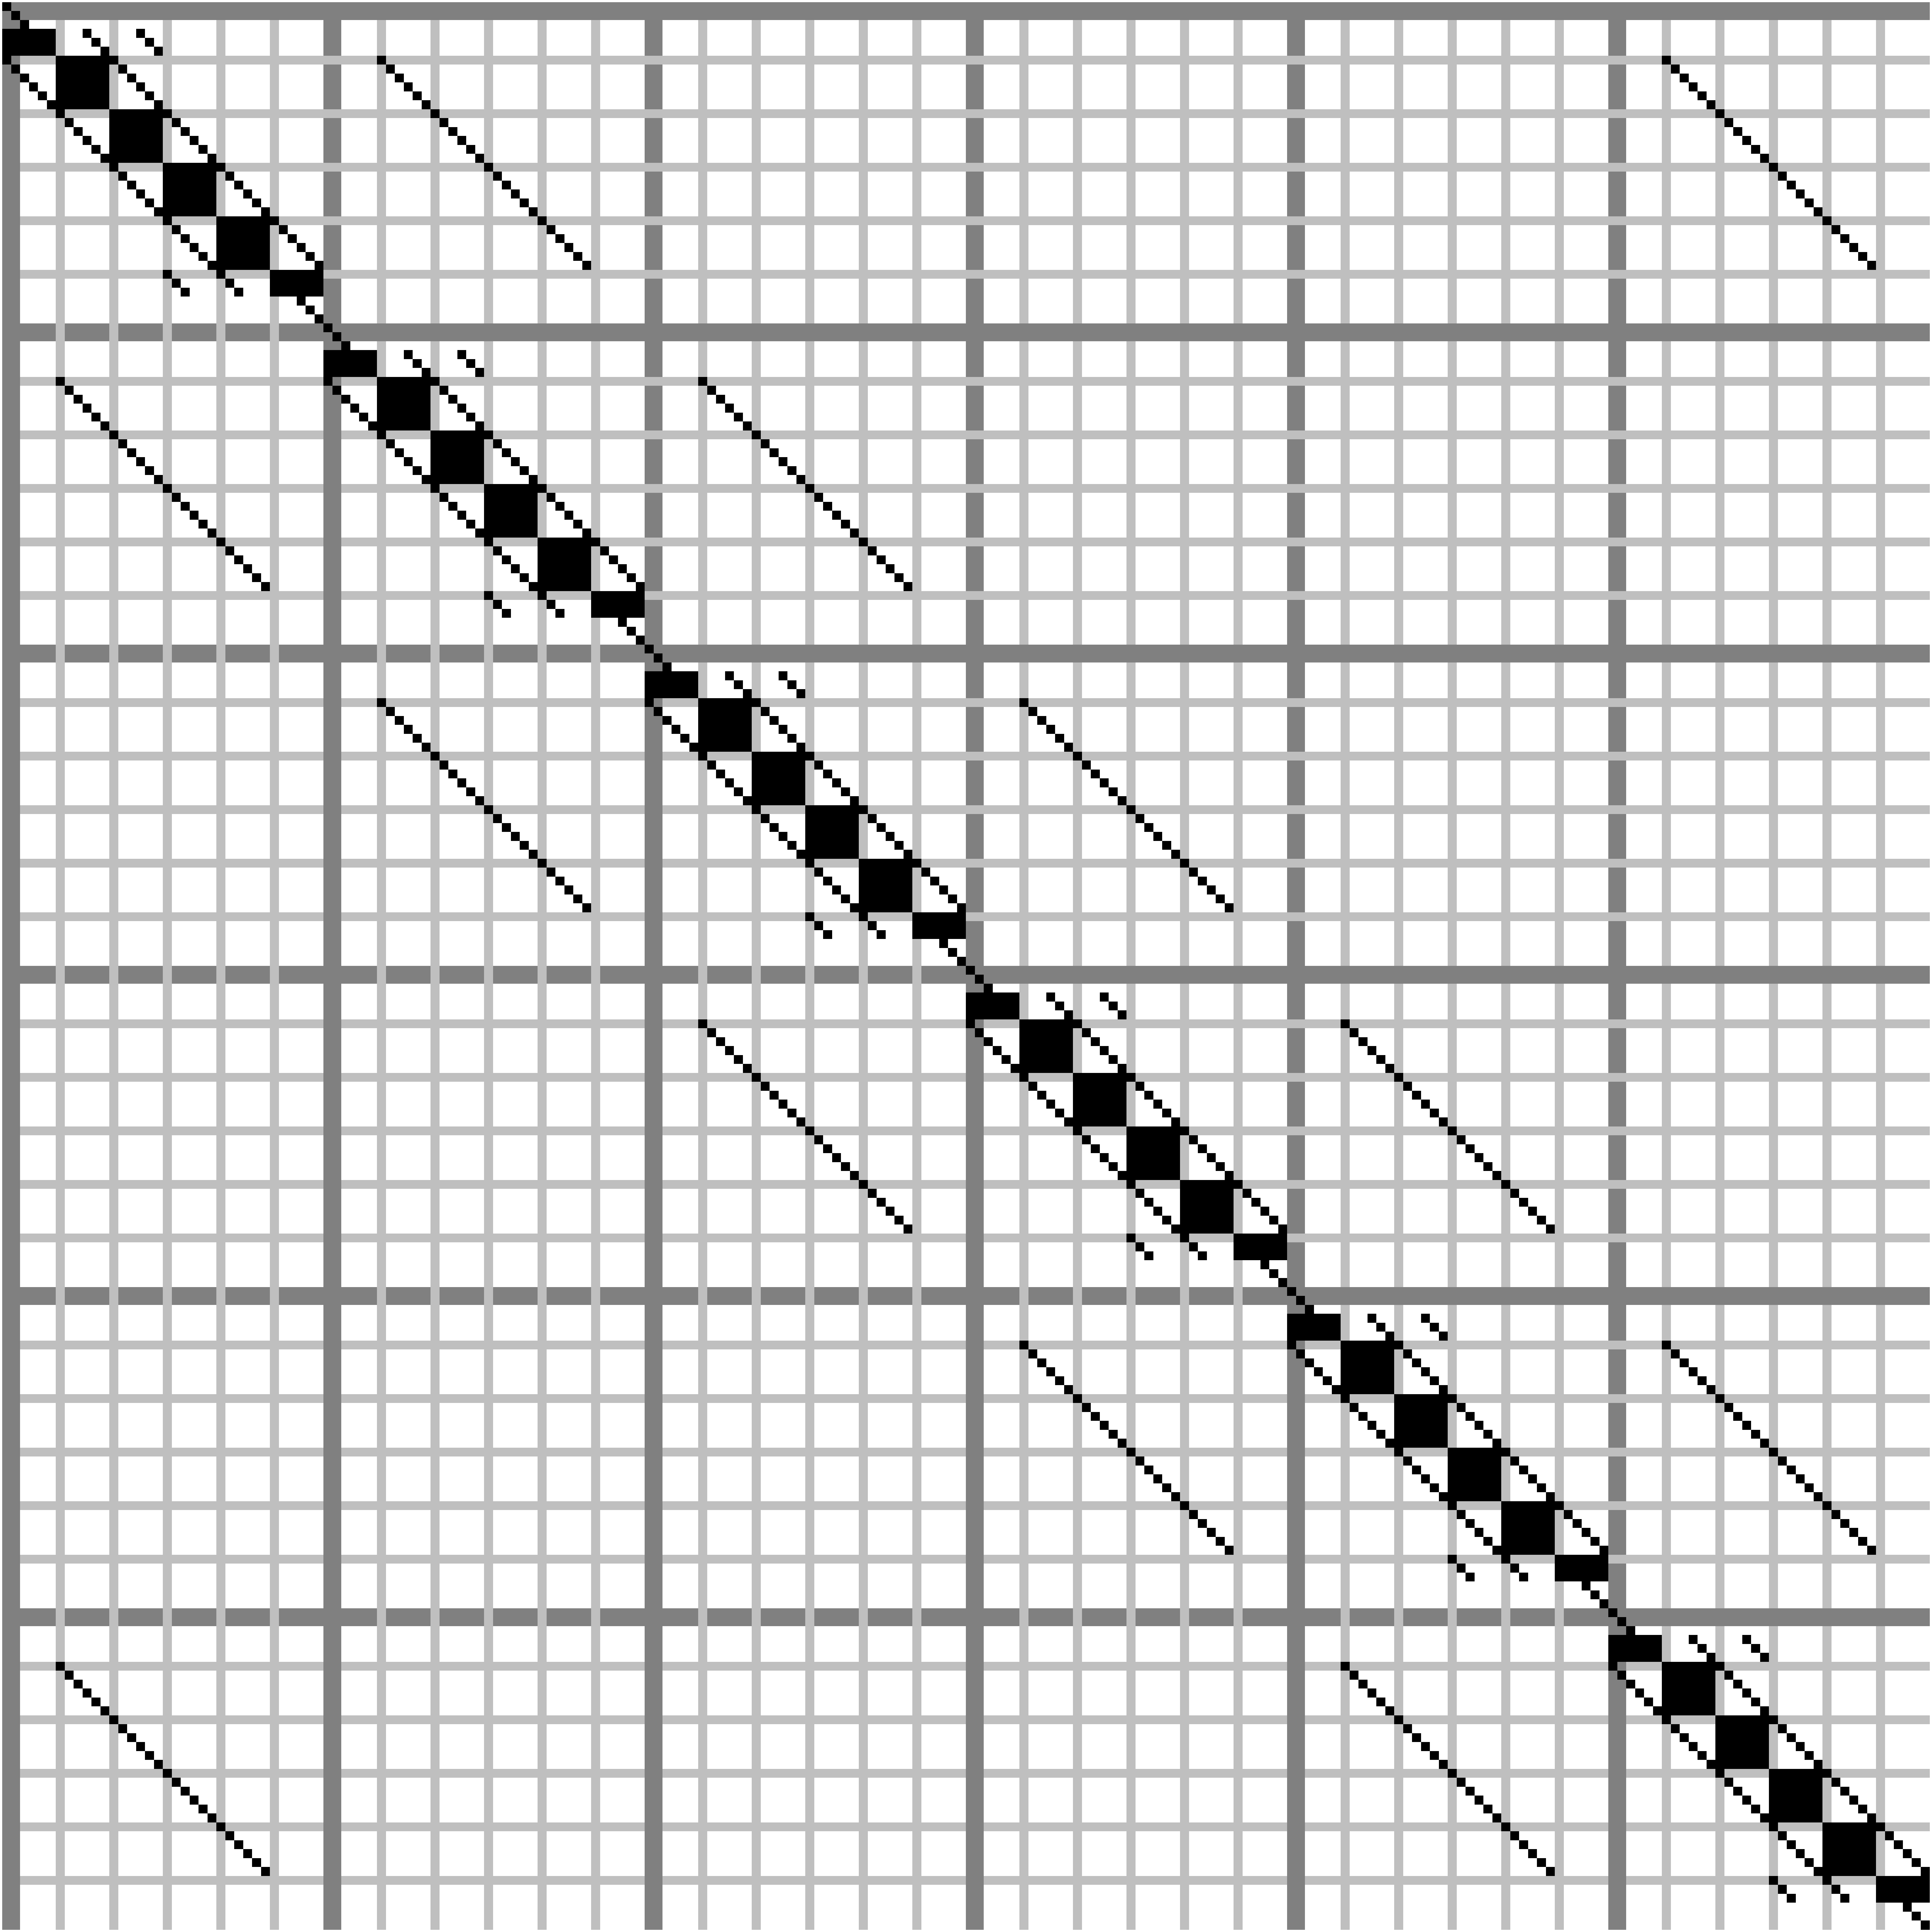
\includegraphics[width=\spwidth]{../img/sparsity/int_small_6x6x6_012.eps}
    \caption{Sparsity plot: 6x6x6, ordering 012 }
\end{figure}
\vspace{\spmgin}
\begin{figure}[H]
    \centering
    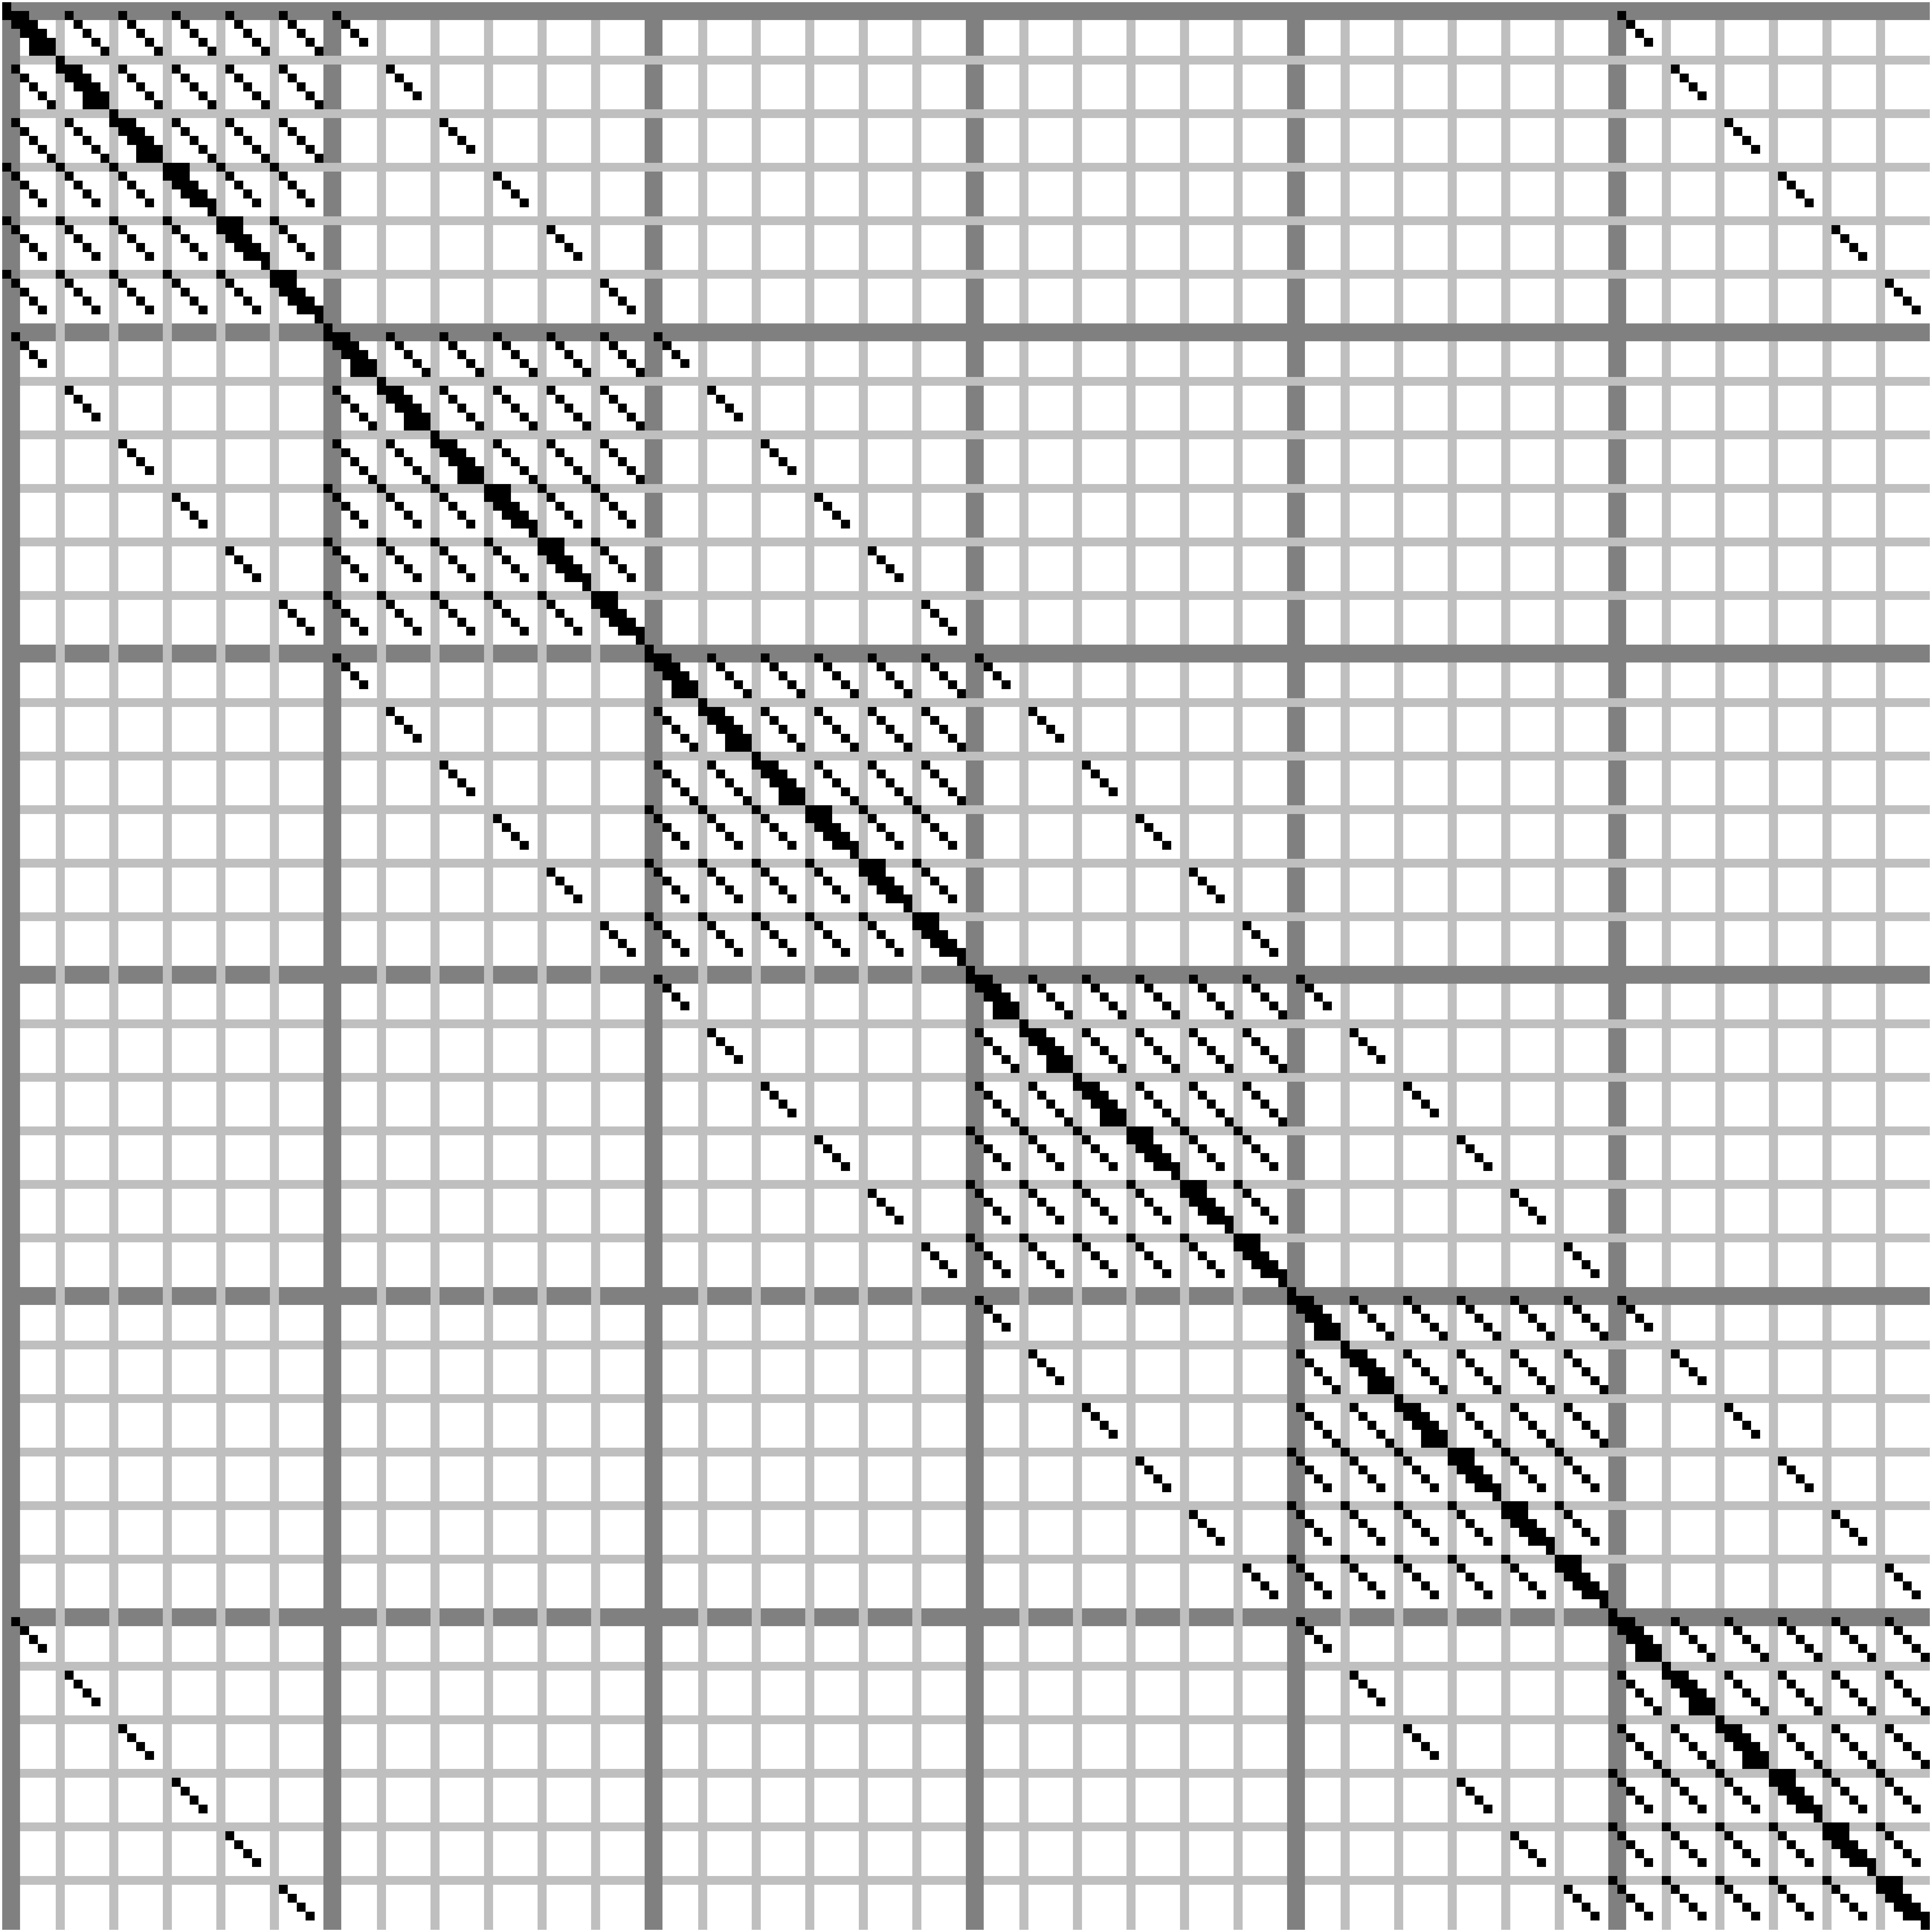
\includegraphics[width=\spwidth]{../img/sparsity/int_small_6x6x6_021.eps}
    \caption{Sparsity plot: 6x6x6, ordering 021 }
\end{figure}
\vspace{\spmgin}
\begin{figure}[H]
    \centering
    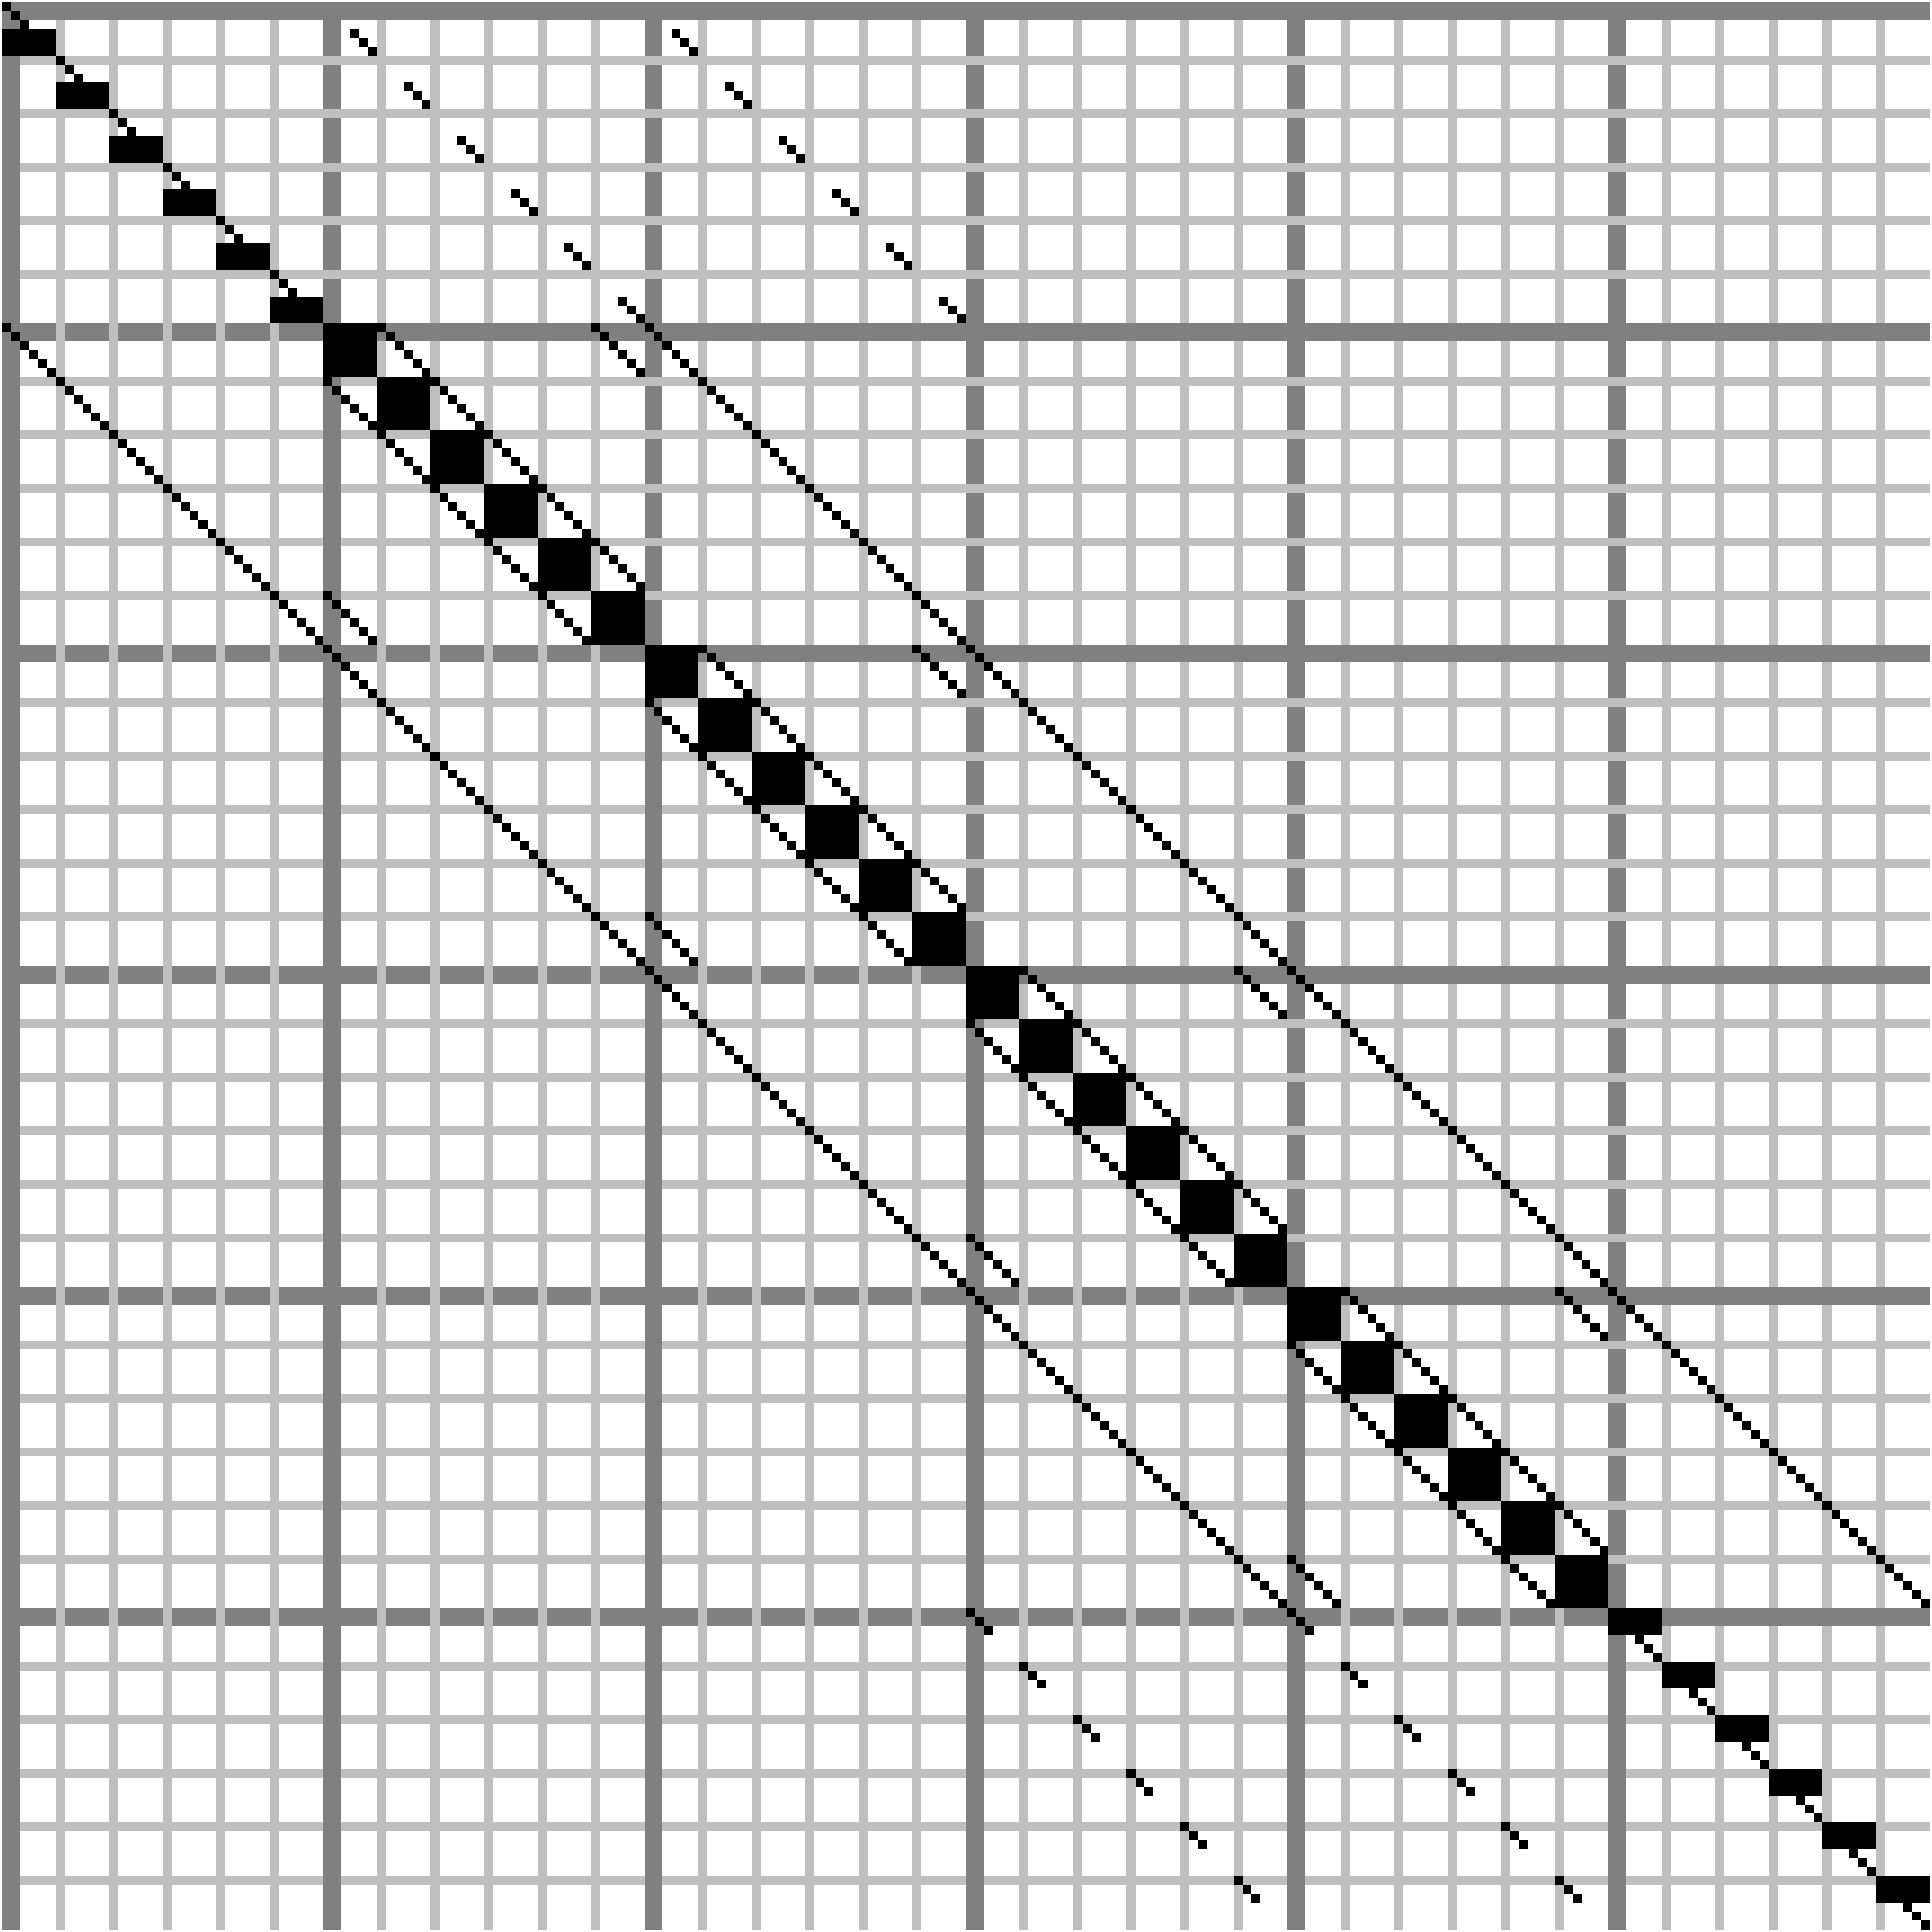
\includegraphics[width=\spwidth]{../img/sparsity/int_small_6x6x6_102.eps}
    \caption{Sparsity plot: 6x6x6, ordering 102 }
\end{figure}
\end{minipage}%
\begin{minipage}[t]{.5\textwidth}%
\begin{figure}[H]
    \centering
    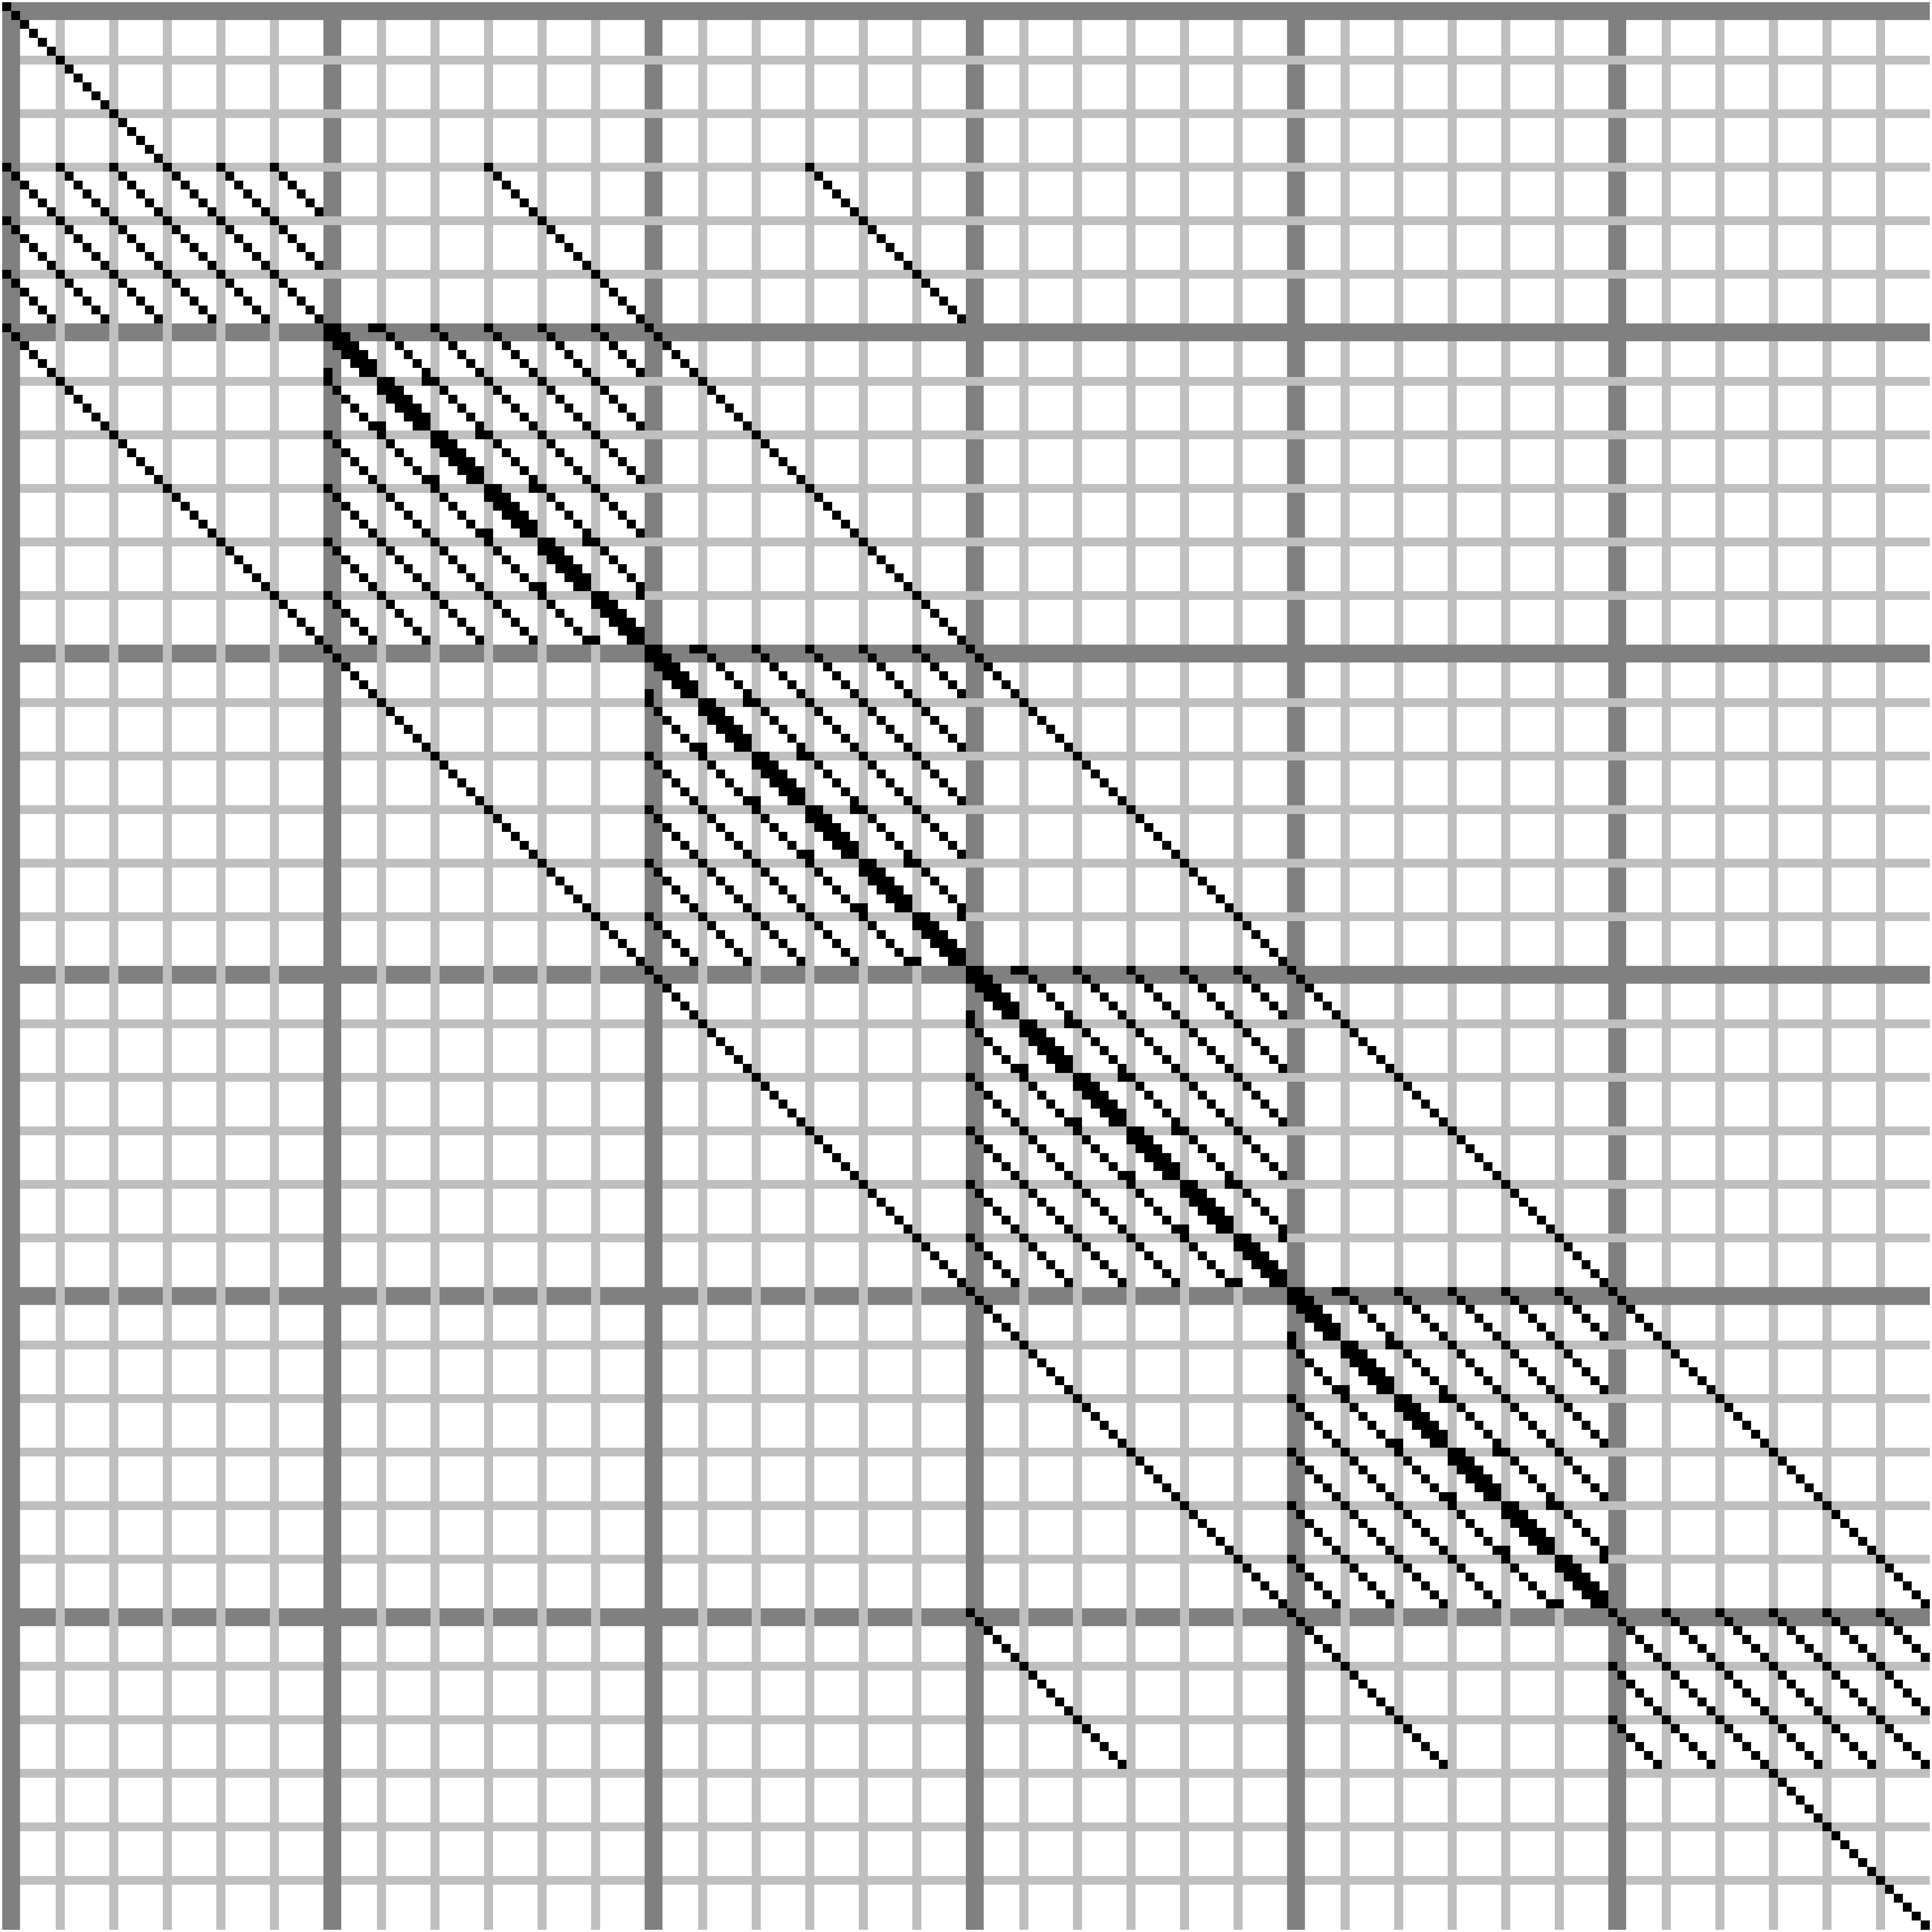
\includegraphics[width=\spwidth]{../img/sparsity/int_small_6x6x6_120.eps}
    \caption{Sparsity plot: 6x6x6, ordering 120 }
\end{figure}
\vspace{\spmgin}
\begin{figure}[H]
    \centering
    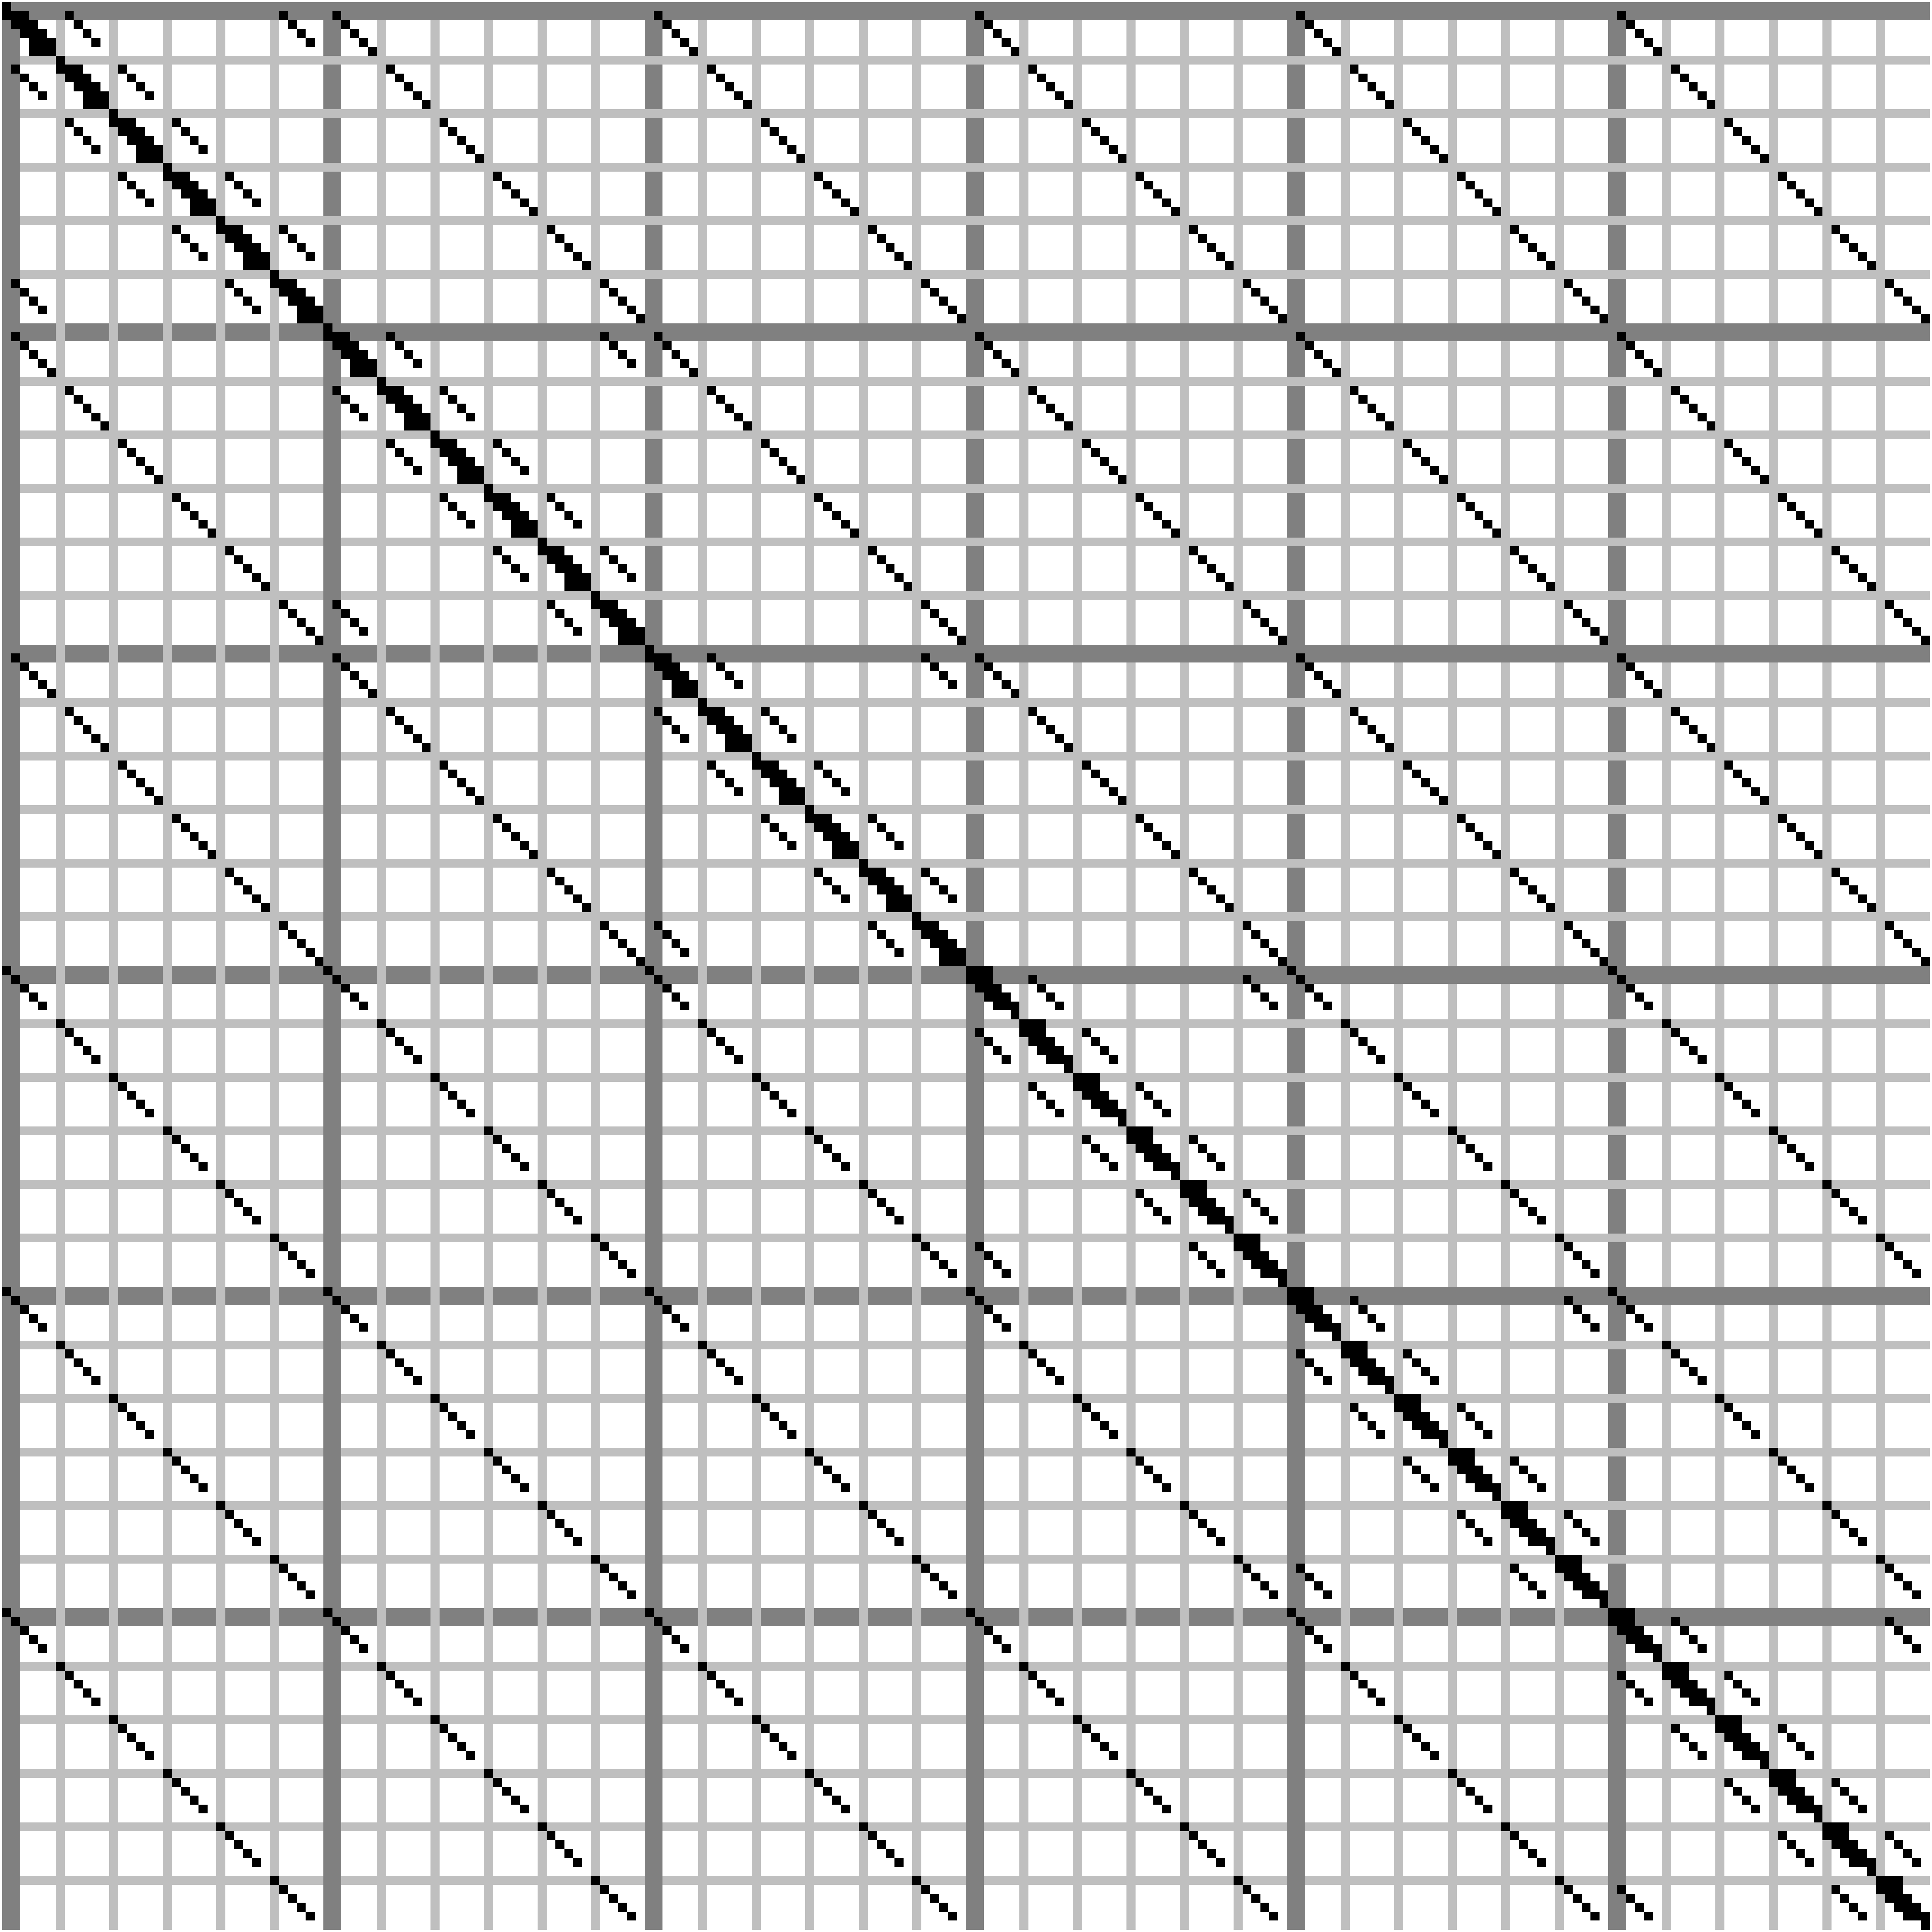
\includegraphics[width=\spwidth]{../img/sparsity/int_small_6x6x6_201.eps}
    \caption{Sparsity plot: 6x6x6, ordering 201 }
\end{figure}
\vspace{\spmgin}
\begin{figure}[H]
    \centering
    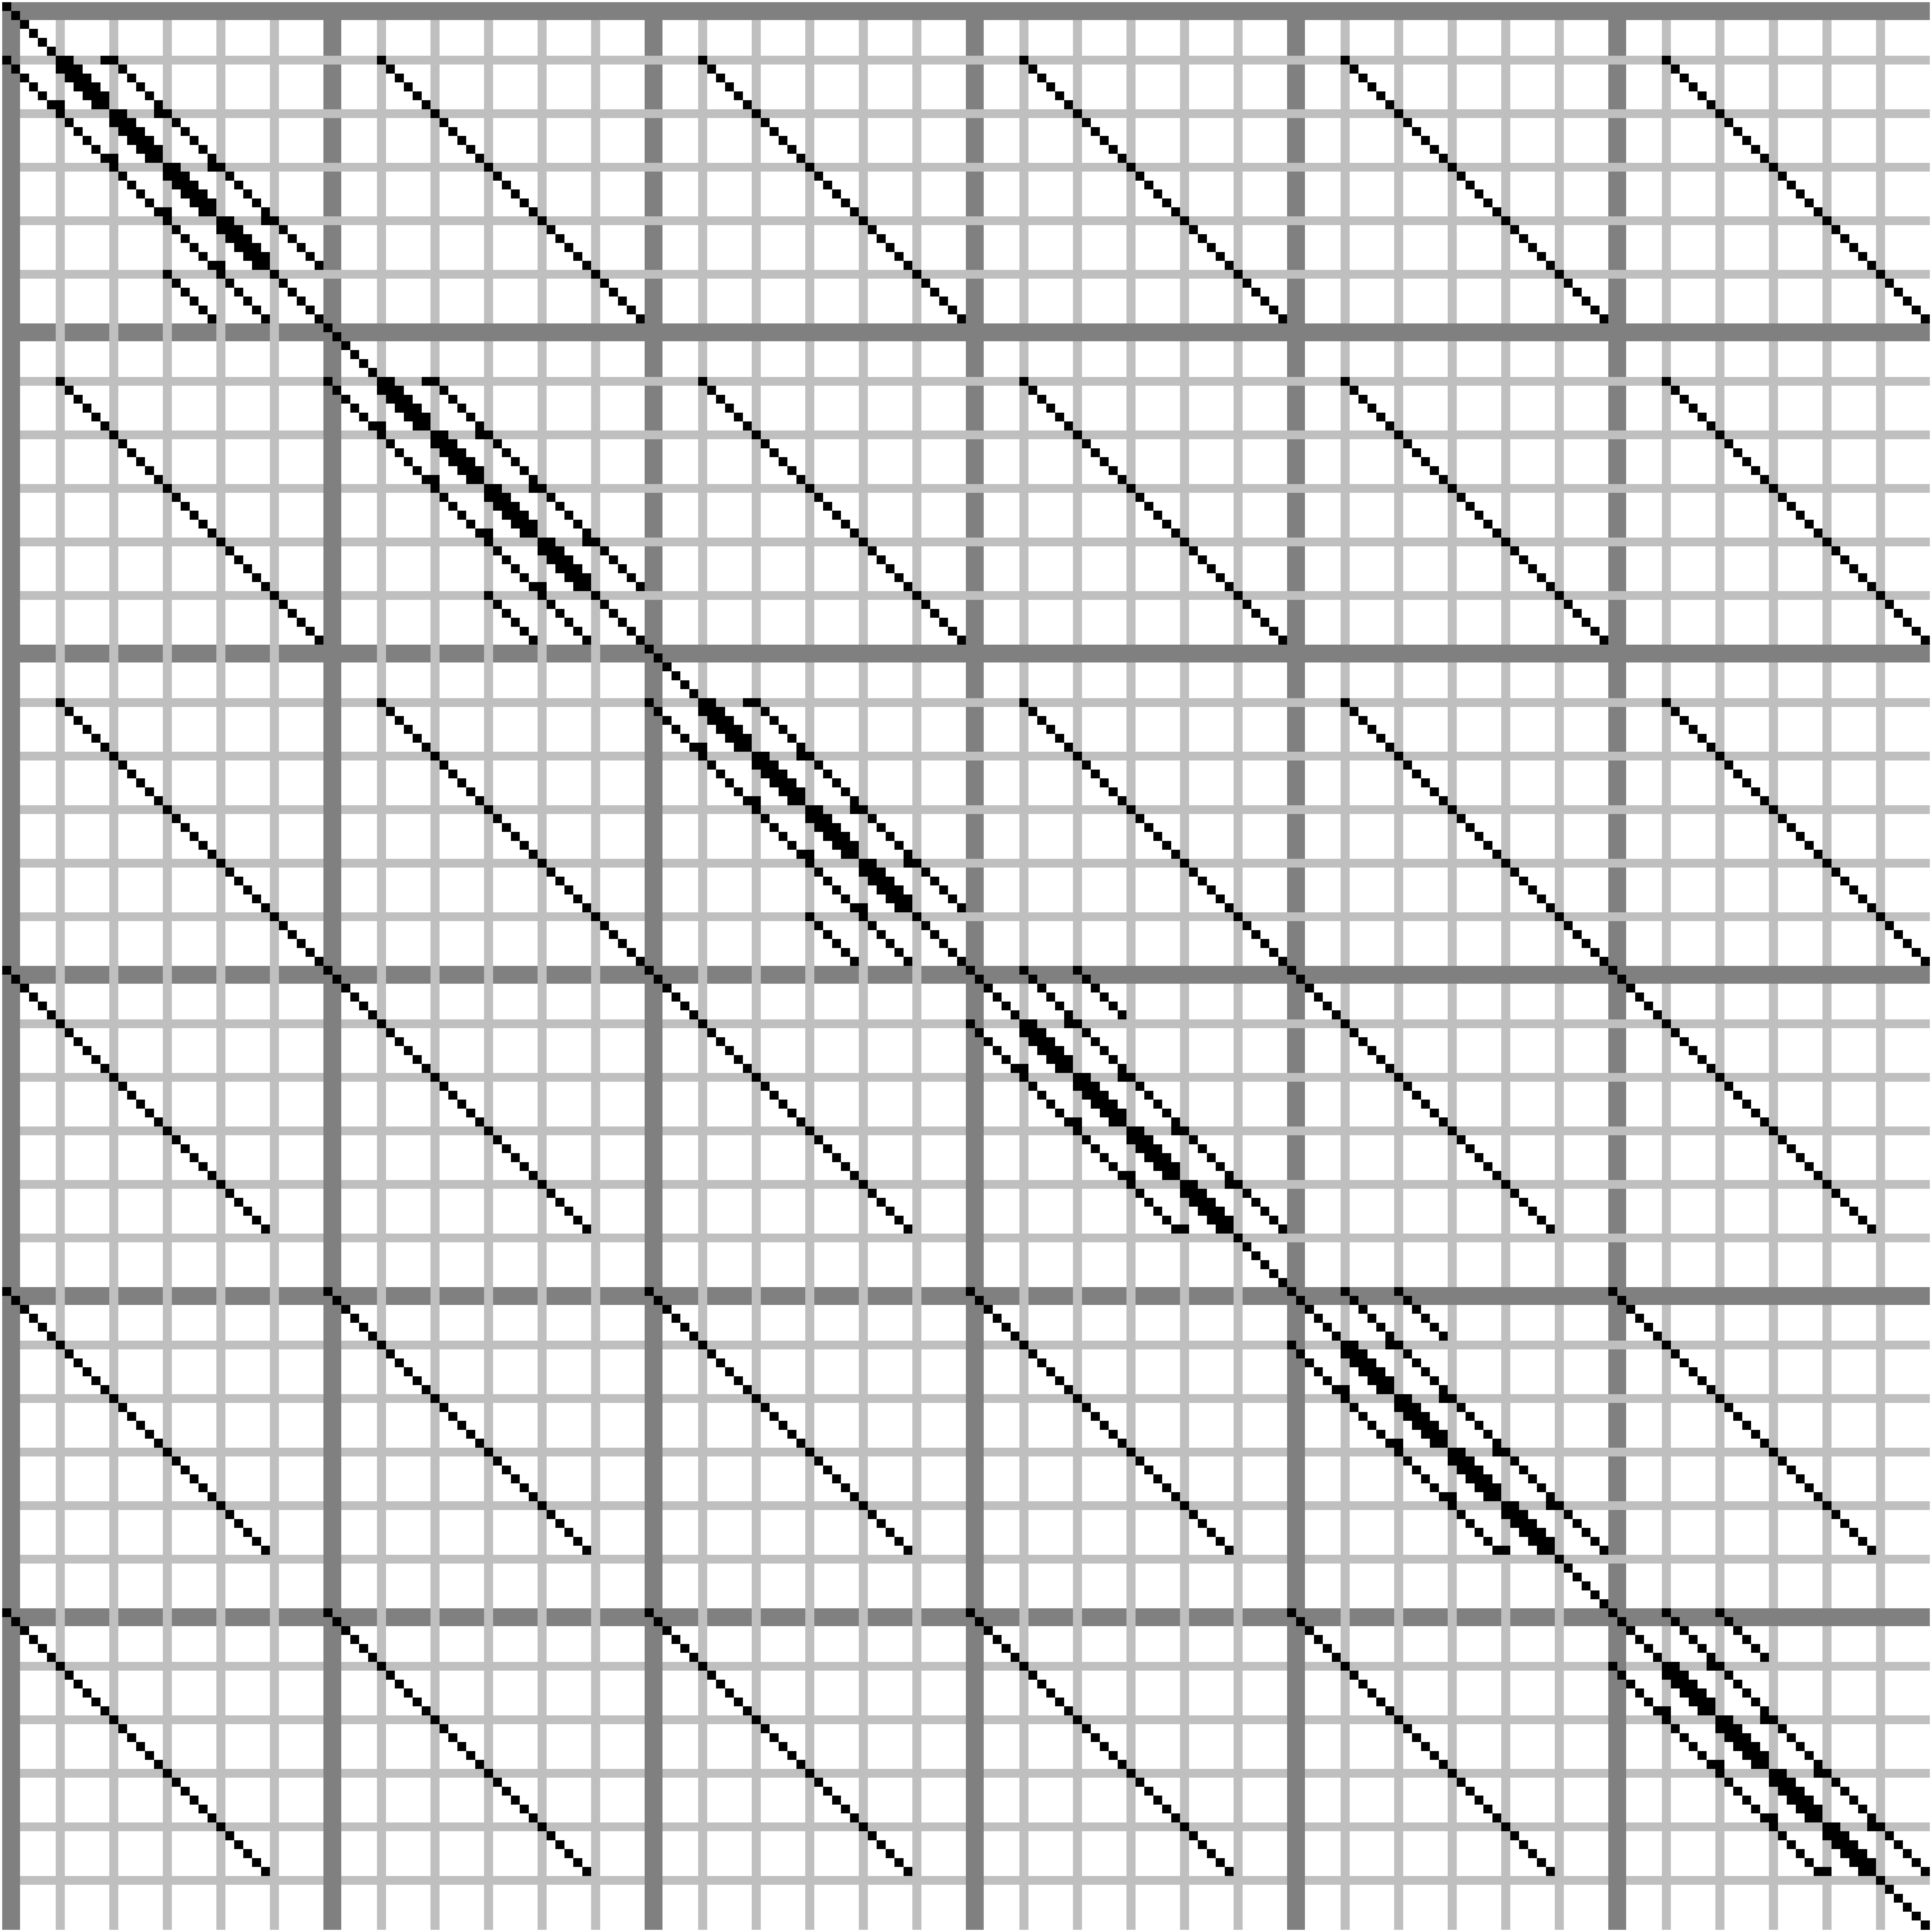
\includegraphics[width=\spwidth]{../img/sparsity/int_small_6x6x6_210.eps}
    \caption{Sparsity plot: 6x6x6, ordering 210 }
\end{figure}
\end{minipage}%
\end{center}
\pagebreak

\subsection{Matrix Properties}
There are several properties which a real matrix can have which simplify or accelerate the solution procedure.
The first is symmetry.
Simply from the sparsity patters, we see that none of the above matrices are symmetric.
A symmetric matrix can additionally be positive definite, in which case numerous highly efficient algorithms exist for solving the system, such as the Conjugate Gradient method \citep{nocedal_numerical_1999}.
Another important property is diagonal dominance.

\subsubsection{Diagonal Dominance}
\label{sec:ddom}

A matrix $A=(a_{ij})$ is said to be diagonally dominant if
\begin{equation}
	\abs{a_{jj}} > \sum_{i\neq j}\abs{a_{ij}} \,\, \mbox{for all}\,\, i \\
\end{equation}

For each $i$, define the quantities
\begin{align}
	\DD_i &= \abs{a_{jj}} \\
	\NN_i &= \sum_{i\neq j}\abs{a_{ij}} \\
	\QQ_i &= \DD_i - \NN_i
\end{align}

Then, $A$ is diagonally dominant if and only if
\begin{equation}
	\min_{1\leq i \leq n} \QQ_i > 0
\end{equation}

\section{Direct Methods}
\subsection{Factorizations}
The most straightforward way to solve any linear system is via Gaussian Elimination, or equivalently, by performing an LU factorization.
However, the number of arithmetic operations required for full LU factorization algorithm grows as $\mathcal{O}(n^3)$, making it impractical for most large systems.
However, specific sparse algorithms exist which discard the zero elements, drastically reducing the computational cost.
Similarly, other factorizations which one might generally use to solve a dense system, such as QR, SVD, and Cholesky have analogous sparse algorithms which ignore all zero elements.

Once a factorization has been computed, solving the system is extremely cheap.
This makes factorization particularly appealing in cases where it is necessary to solve numerous systems with the same coefficient matrix $A$, but for different right-hand side vectors $b$.
This occurs in particular for linear time-dependent PDEs.
However, since we are considering the time-independent RTE, that appeal is lost on us.

Another major limitation of factorizations is the large amount of memory they require.
Fundamentally, factorizations require the storage of multiple factors, which need not necessarily preserve the sparsity pattern of the original matrix.
This limitation is somewhat avoidable with out-of-core computations, whereby matrices are stored directly on the hard drive rather than in memory.
Computations directly on disk, however, are anywhere from 6 to $10^5$ times slower than computations in memory \citep{jacobs_pathologies_2009}.

\subsection{Software Packages}
Many implementations of direct methods exist for particular circumstances.
\texttt{LAPACK} \citep{anderson_lapack_1999}, the well known free and open source \texttt{FORTRAN} linear algebra library, contains subroutines for banded, triangular, symmetric, tridiagonal, and general matrices.
Of those, the banded solver is potentially applicable to the system we consider.
A variety of more sophisticated free and open source packages for solving sparse systems directly exist, such as \texttt{UMFPACK} \citep{davis_algorithm_2004} and \texttt{MUMPS} \citep{amestoy_mumps:_2001}.
Both of these algorithms in particular are \textit{multi-frontal}, which is to say that they only keep small slices (fronts) of the matrix in memory at any given time, and perform computations on several fronts in parallel, drastically reducing solution time.

\section{Stationary Iterative Methods}
\subsection{Fixed-Point Iteration}
Iterative methods are another way in which to solve linear systems of equations.
Iterative methods work to successively improve upon their approximate solution, stopping when the results are calculated to within a tolerance which can be set as desired.
Iterative methods are a generally good option for solving a linear system $Ax=b$ particularly when $A$ is large.
Since these systems meet that criteria, this was a path that was desirable to explore to see how these results compared.


We follow \citet[Section 1.1]{anderson_analysis_2012} in describing basic Stationary Iterative Methods operate as follows.
Given $Ax = b$, we choose $N$ and $P$ such that 
\begin{equation}
	A = N-P,
	\label{eq:it_split}
\end{equation}
where $N$ is invertible.

Then,
\begin{align*}
    Ax &= b \\
    (N-P)x &= b \\
    Nx &= Px + b
\end{align*}

Extending the idea of fixed point iteration to systems, we take the two instances of $x$ in the above equation to be consecutive iterates, and obtain
\begin{equation}
    x\iter{i+1} = N^{-1}Px\iter{i} + N^{-1}b
    \label{eq:it_np}
\end{equation}

Letting $G=N^{-1}P$ and $C=N^{-1}b$, we have the general form
\begin{equation}
    x\iter{i+1} = Gx\iter{i} + C
    \label{eq:it_g}
\end{equation}

The choice of $N$ and $P$ in the above equations determine the particular Stationary Iterative Method.
In fact, given that the two are related by \eqref{eq:it_split}, the choice of $N$ uniquely defines a method.

The most common methods are listed here, where $D$, $L$, and $U$ represent the diagonal, strictly lower triangular, and strictly upper triangular pieces of $A$ respectively, $I$ is the identity matrix, $\omega$ and $p$ are free parameters for which the optimal value is problem-dependent.

\begin{figure}[H]
	\centering
	\begin{tabular}{ll}
		\toprule
		Method & $N$ \\
		\midrule
		Jacobi & $D$ \\
		JOR & $\frac{1}{\omega}D$ \\
		Gauss-Seidel & $D + L$ \\
		SOR & $\frac{1}{\omega}D + L$ \\
		Richardson & $-\frac{1}{p}I$ \\
		\bottomrule
	\end{tabular}
	\caption{Basic Linear Stationary Iterative Methods \citep{young_iterative_1971}}
\end{figure}


%There are two types of iterative methods in general and these are Stationary and Krylov subspace.
%The first of these to be explored were the Stationary methods.
%Stationary iterative methods can be expressed in the general form:

%where the $x$ values change from iteration to iteration while $G$ and $C$ remain constant.
%A general advantage of these methods are that they are simple to derive, implement and analyze.
%The disadvantage is that convergence is not guaranteed and for most real-world type problems would not be anticipated.

%Two types of Stationary Iterative methods were explored for these systems, the Jacobi and Gauss-Seidel methods.
%As these methods were described in detail within the scope of the Advanced Numerical Analysis II coursework, these will not be explored in detail.
%Code was developed to implement these algorithms as discussed in the class.

\subsection{Convergence (or lack thereof)}

It is a well-known result \citep{anderson_analysis_2012} that the iterative method defined by \eqref{eq:it_g} converges to the exact solution $x$ if and only if $\rho(G) < 1$, where $\rho(G)$ is the \textit{spectral radius} of $G$, defined as the largest magnitude of an eigenvalue of $G$.
A sufficient but unnecessary condition for convergence of \eqref{eq:it_g} is the diagonal dominance of $A$.

As we observed in section \ref{sec:ddom}, $A$ is in general not diagonally dominant for this problem.
Further, we show that it's eigenvalues need not be bounded in the unit circle.

\subsubsection{Gershgorin Disks}


% Since the systems would not be guaranteed to converge and there were numerous orderings and resolutions, creating systems that ranged from large to very large, it was helpful to save time to know whether convergence would be expected in advance.
% There were two ways to do this.
% First was to check diagonal dominance.
% Code was developed for this check and resulted in none of the systems having this property.
% However, this was not a necessary criteria so something more specific was desired.
% 
% One of the properties of iterative systems is that it is possible to take the eigenvalues of $G$ (with the system in the general form).
% For any initial guess of $x$, it can be proven that the problem converges if and only if those eigenvalues all lie within the unit circle.
% Code was developed to check this property and ran approximately ten times faster than directly running just a few iterations of the methods directly.
% This was a significant cost savings for larger matrices.
% Unfortunately, the conclusion was that none of the initial matrices would converge through either method under study.

\subsubsection{Preconditioning}

Although the matrix is not naturally suited for stationary iterative methods, it is possible to precondition the matrix in order to induce diagonal dominance.
We consider two such preconditioning strategies.

The first option is the computation of the SVD of $A$, using $U$ and $V^T$ as preconditioners.
However, given the large computational cost of SVD and the lack of readily available efficient sparse algorithms, this was deemed infeasible.

We did, though, explore the method of Jacobi iterations discussed in \citet{yuan_method_2006} to identify and gradually reduce the off-diagonal terms.
This serves to make the system increasingly diagonally dominant until becoming solvable with Stationary Iterative Methods.
 
Our implementation of the Jacobi iteration algorithm successfully preconditioned the matrix corresponding to a $10\times 16$ spatial-angular grid for diagonal dominance, however the time required for preconditioning was on the order of hours, whereas the time required to solve directly or by a nonstationary iterative method was on the order of seconds.
Clearly, this is an inappropriate approach for our problem.
Nonetheless, after preconditioning, both Jacobi and Gauss-Seidel iteration were successfully executed with a tolerance of \texttt{1e-3} and an initial guess of the zero vector.

\begin{figure}[H]
	\centering
	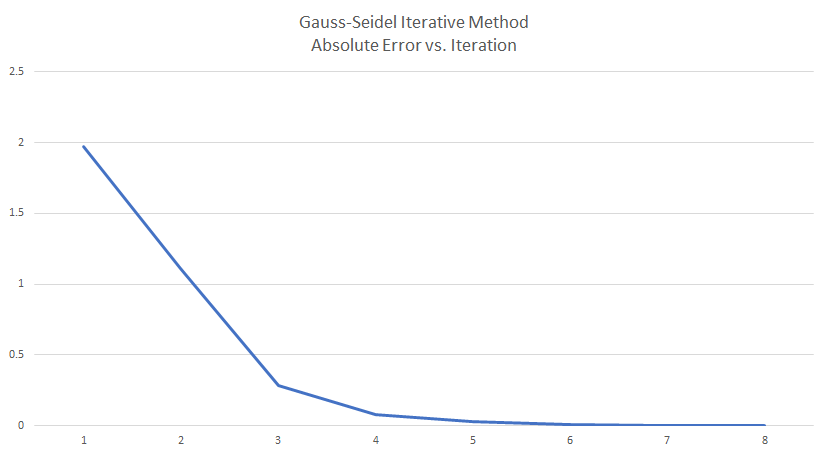
\includegraphics[width=3.5in]{../img/fred_stat_it/img1.png}
	\caption{The Jacobi method ran in 47 iterations, taking a total computation time of 3.85 seconds.}
\end{figure}

\begin{figure}[H]
	\centering
	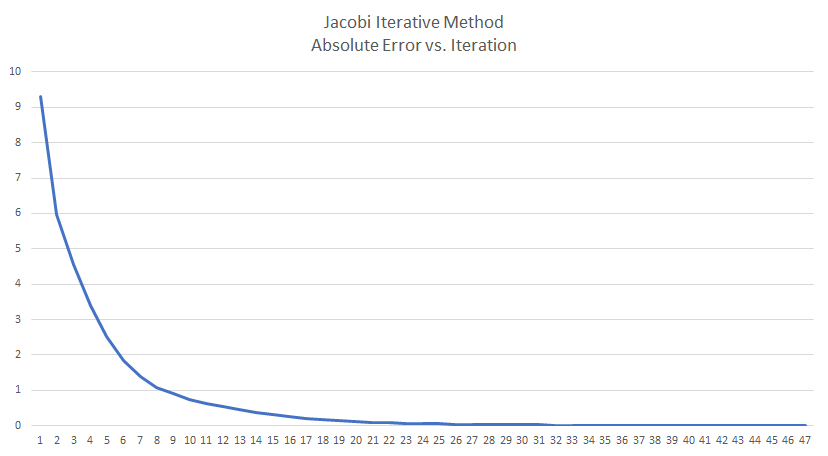
\includegraphics[width=3.5in]{../img/fred_stat_it/img2.png}
	\caption{GS method completed in 8 iterations and taking a total time of 0.75 seconds.}
\end{figure}

In this case, the Gauss-Seidel method was faster and less expensive than Jacobi.
It is also worth noting that fewer Jacobi iterations were necessary in the preconditioning process to allow the Gauss-Seidel method to begin to converge, further making this method more effective for this particular system.

\section{Nonstationary Methods}
Clearly, both direct methods and Stationary Iterative Methods have significant limitations in their ability to solve large sparse systems arising from general multidimensional PDEs.
Enter nonstationary methods.
A nonstationary iterative method is any iterative method which does not have the form \eqref{eq:it_g}.
Generally, though, the most common nonstationary methods are Krylov Subspace methods, which is a class of methods that have become increasingly popular in recent decades due to their flexibility and speed \citep{gutknecht_brief_2007}.

\subsection{Krylov Subspace Methods}

The $k^{th}$ Krylov Subspace generated by a matrix $A \in \mathbb{R}^{n\times n}$ and a vector $v \in \mathbb{R}^n$ is defined as
\begin{equation}
	K_k(A,v) = \mbox{span}\left\{A^iv\right\}_{i=0}^{i=k-1}
\end{equation}

The general approach of a Krylov Subspace method is to successively generate Krylov Subspaces by constructing basis vectors for them, and to find the vector contained in each subspace with the minimum residual $r = \norm{Ax-b}$
These basis vectors are usually generated with either Arnoldi iteration or bi-Lanczos iteration, both of which apply variants of the Gram-Schmidt orthogonalization process \citep{ghai_comparison_2016}.

The Krylov subspace methods we consider are \texttt{GMRES}, \texttt{LGMRES}, \texttt{BiCG}, \texttt{BiCGSTAB}, \texttt{QMR}, and \texttt{CGS}.
Two other well known Krylov Subspace Methods are \texttt{CG} and \texttt{MINRES}, although they are applicable only to symmetric positive definite systems.

\subsection{Convergence and Preconditioning}
Unlike nonstationary methods for symmetric positive definite matrices, the convergence properties of GMRES, BiCG and other nonsymmetric nonstationary methods are not well understood.
Generally, performance tends to worsen with increasing condition number and improve with increasing eigenvalue clustering.
Preconditioners are very commonly used with Krylov Subspace methods to improve the system in these two regards.

%% Citations??
\subsubsection{Eigenvalue Clustering}

\section{Numerical Results}

\section{Conclusions}

%\nocite{*}
\bibliographystyle{abbrvnat}
\bibliography{rte_matrix_report}
\end{multicols}
\end{document}


